%%%%%%%%%%%%%%%%%%%%%%%%%%%%%%%%%%%%%%%%%%%%%%%%%%%%%%%%%%%%%%%%%%%%%%%%%%%%%%%%
%% Plantilla de memoria en LaTeX para la ETSIT - Universidad Rey Juan Carlos
%%
%% Por Gregorio Robles <grex arroba gsyc.urjc.es>
%%     Grupo de Sistemas y Comunicaciones
%%     Escuela Técnica Superior de Ingenieros de Telecomunicación
%%     Universidad Rey Juan Carlos
%% (muchas ideas tomadas de Internet, colegas del GSyC, antiguos alumnos...
%%  etc. Muchas gracias a todos)
%%
%% La última versión de esta plantilla está siempre disponible en:
%%     https://github.com/gregoriorobles/plantilla-memoria
%%
%% Para obtener PDF, ejecuta en la shell:
%%   make
%% (las imágenes deben ir en PNG o JPG)

%% Adaptado para la ETSII por Marcos Tenrero <tenrero@aol.com>

%%%%%%%%%%%%%%%%%%%%%%%%%%%%%%%%%%%%%%%%%%%%%%%%%%%%%%%%%%%%%%%%%%%%%%%%%%%%%%%%

\documentclass[a4paper, 12pt]{book}
%\usepackage[T1]{fontenc}

\usepackage[a4paper, left=2.5cm, right=2.5cm, top=3cm, bottom=3cm]{geometry}
\usepackage{times}
\usepackage[utf8]{inputenc}
\usepackage[T1]{fontenc}
\usepackage[spanish]{babel}
\usepackage{hyperref}
%\usepackage[dvipdfm]{graphicx}
\usepackage{graphicx}
\usepackage{float}  %% H para posicionar figuras
\usepackage[nottoc, notlot, notlof, notindex]{tocbibind} %% Opciones de índice
\usepackage{latexsym}  %% Logo LaTeX
\usepackage{float}

\title{Memoria del Proyecto}
\author{Nombre del autor}

\renewcommand{\baselinestretch}{1.5}  %% Interlineado

\begin{document}

\renewcommand{\refname}{Bibliografía}  %% Renombrando
\renewcommand{\appendixname}{Apéndice}

%%%%%%%%%%%%%%%%%%%%%%%%%%%%%%%%%%%%%%%%%%%%%%%%%%%%%%%%%%%%%%%%%%%%%%%%%%%%%%%%
% PORTADA

\begin{titlepage}
\begin{center}
\begin{tabular}[c]{c c}
%\includegraphics[bb=0 0 194 352, scale=0.25]{logo} &
\includegraphics[scale=0.25]{img/logo_vect.png} &
\begin{tabular}[b]{l}
\Huge
\textsf{UNIVERSIDAD} \\
\Huge
\textsf{REY JUAN CARLOS} \\
\end{tabular}
\\
\end{tabular}

\vspace{3cm}

\Large
TITULACIÓN EN MAYÚSCULAS

\vspace{0.4cm}

\large
Curso Académico 20XX/20XX

\vspace{0.8cm}

Trabajo Fin de Grado/Máster

\vspace{2.5cm}

\LARGE
TÍTULO DEL TRABAJO EN MAYÚSCULAS

\vspace{4cm}

\large
Autor : Nombre del Alumno/a \\
Tutor : Nombre del Tutor del TFG
\end{center}
\end{titlepage}

\newpage
\mbox{}
\thispagestyle{empty} % para que no se numere esta página


%%%%%%%%%%%%%%%%%%%%%%%%%%%%%%%%%%%%%%%%%%%%%%%%%%%%%%%%%%%%%%%%%%%%%%%%%%%%%%%%
%%%% Para firmar
\clearpage
\pagenumbering{gobble}
\chapter*{}

\vspace{-4cm}
\begin{center}
\LARGE
\textbf{Trabajo Fin de Grado/Máster}

\vspace{1cm}
\large
Título del Trabajo con Letras Capitales para Sustantivos y Adjetivos

\vspace{1cm}
\large
\textbf{Autor :} Nombre del Alumno/a \\
\textbf{Tutor :} Nombre del Tutor del TFG

\end{center}

\vspace{1cm}
La defensa del presente Proyecto Fin de Carrera se realizó el día \qquad$\;\,$ de \qquad\qquad\qquad\qquad \newline de 20XX, siendo calificada por el siguiente tribunal:


\vspace{0.5cm}
\textbf{Presidente:}

\vspace{1.2cm}
\textbf{Secretario:}

\vspace{1.2cm}
\textbf{Vocal:}


\vspace{1.2cm}
y habiendo obtenido la siguiente calificación:

\vspace{1cm}
\textbf{Calificación:}


\vspace{1cm}
\begin{flushright}
Fuenlabrada, a \qquad$\;\,$ de \qquad\qquad\qquad\qquad de 20XX
\end{flushright}

%%%%%%%%%%%%%%%%%%%%%%%%%%%%%%%%%%%%%%%%%%%%%%%%%%%%%%%%%%%%%%%%%%%%%%%%%%%%%%%%
%%%% Dedicatoria

\chapter*{}
\pagenumbering{Roman} % para comenzar la numeración de páginas en números romanos
\begin{flushright}
\textit{Dedicado a \\
mi familia / mi abuelo / mi abuela}
\end{flushright}

%%%%%%%%%%%%%%%%%%%%%%%%%%%%%%%%%%%%%%%%%%%%%%%%%%%%%%%%%%%%%%%%%%%%%%%%%%%%%%%%
%%%% Agradecimientos

\chapter*{Agradecimientos}
%\addcontentsline{toc}{chapter}{Agradecimientos} % si queremos que aparezca en el índice
\markboth{AGRADECIMIENTOS}{AGRADECIMIENTOS} % encabezado

Aquí vienen los agradecimientos\ldots Aunque esté bien acordarse de la pareja, no hay que olvidarse de dar las gracias a tu madre, que aunque a veces no lo parezca disfrutará tanto de tus logros como tú\ldots
Además, la pareja quizás no sea para siempre, pero tu madre sí.

%%%%%%%%%%%%%%%%%%%%%%%%%%%%%%%%%%%%%%%%%%%%%%%%%%%%%%%%%%%%%%%%%%%%%%%%%%%%%%%%
%%%% Resumen

\chapter*{Resumen}
%\addcontentsline{toc}{chapter}{Resumen} % si queremos que aparezca en el �ndice
\markboth{RESUMEN}{RESUMEN} % encabezado

Aqu� viene un resumen del proyecto. Ha de constar de tres o cuatro p�rrafos, donde se presente de manera clara y concisa de qu� va el proyecto. 
Han de quedar respondidas las siguientes preguntas:

\begin{itemize}
  \item �De qu� va este proyecto? �Cu�l es su objetivo principal?
  \item �C�mo se ha realizado? �Qu� tecnolog�as est�n involucradas?
  \item �En qu� contexto se ha realizado el proyecto? �Es un proyecto
dentro de un marco general?
\end{itemize}

Lo mejor es escribir el resumen al final.

%%%%%%%%%%%%%%%%%%%%%%%%%%%%%%%%%%%%%%%%%%%%%%%%%%%%%%%%%%%%%%%%%%%%%%%%%%%%%%%%
%%%%%%%%%%%%%%%%%%%%%%%%%%%%%%%%%%%%%%%%%%%%%%%%%%%%%%%%%%%%%%%%%%%%%%%%%%%%%%%%
% ÍNDICES %
%%%%%%%%%%%%%%%%%%%%%%%%%%%%%%%%%%%%%%%%%%%%%%%%%%%%%%%%%%%%%%%%%%%%%%%%%%%%%%%%

%%%% Índice de contenidos
\tableofcontents
%%%% Índice de figuras
\cleardoublepage
%\addcontentsline{toc}{chapter}{Lista de figuras} % para que aparezca en el índice de contenidos
\listoffigures
%%%% Índice de tablas
%\cleardoublepage
%\addcontentsline{toc}{chapter}{Lista de tablas}
%\listoftables

%%%%%%%%%%%%%%%%%%%%%%%%%%%%%%%%%%%%%%%%%%%%%%%%%%%%%%%%%%%%%%%%%%%%%%%%%%%%%%%%
% INTRODUCCIÓN Y MOTIVACIÓN %
%%%%%%%%%%%%%%%%%%%%%%%%%%%%%%%%%%%%%%%%%%%%%%%%%%%%%%%%%%%%%%%%%%%%%%%%%%%%%%%%

\cleardoublepage
\chapter{Introducción y Motivación}
\label{sec:intro} % etiqueta para poder referenciar luego en el texto con ~\ref{sec:intro}
\pagenumbering{arabic} % para empezar la numeración de página con números

% Contexto en el que se enmarca el proyecto y la justificación del mismo. Este capítulo es muy importante porque permite al lector conocer qué sentido tiene el proyecto, qué ofrece, por qué es relevante su implementación, los objetivos que persigue, etc. Este capítulo debería tener una extensión de entre 4 y 8 páginas.

\section{Mercado actual de las aplicaciones móviles}

Las aplicaciones móviles han transformado por completo nuestro día  a día y tienen un gran impacto en cómo nos comunicamos, cómo trabajamos, cómo nos divertimos y cómo realizamos nuestras tareas.

Entre esas tareas se encuentra realizar la compra del hogar, tarea que requiere de organización si el usuario quiere realizarla de manera óptima. Este trabajo de fin de grado se enfoca en generar una herramienta que sirva de ayuda para que los usuarios la lleven a cabo. A partir de este momento, la aplicación que se desarrolla a lo largo de este proyecto la llamaremos \textbf{Pinche}.

Según los datos de 42matters, compañía que se encarga de recopilar y ofrecer datos a diferentes empresas, a 27 de enero de 2024 hay 2 millones aplicaciones Android en Google Play y algo más de 1.900.000 aplicaciones iOS en App Store, Figura~\ref{fig:apps_free_vs_pay}. De las cuales, el porcentaje de aplicaciones que los usuarios se pueden descargar de manera gratuita es aproximadamente de 95\% en ambas tiendas de aplicaciones.

\begin{figure}[H]
\centering
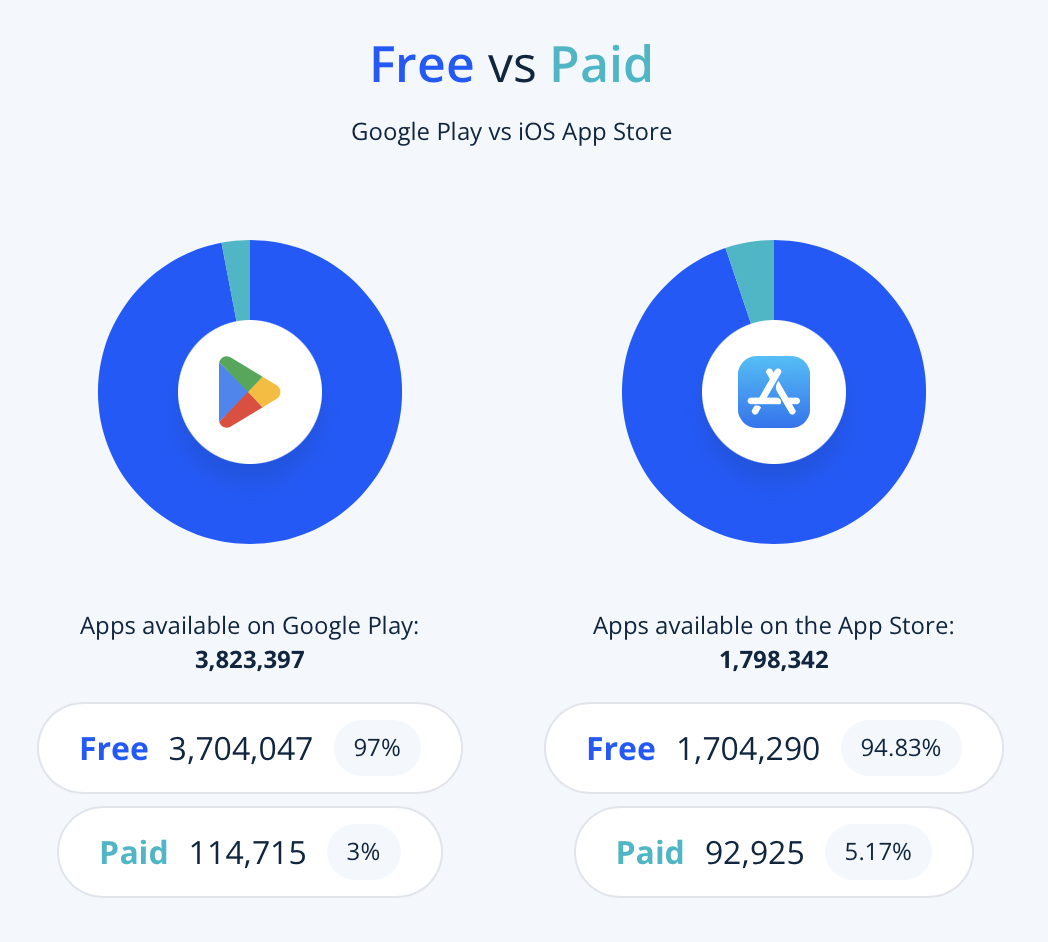
\includegraphics[width=0.6\textwidth]{./img/intro/apps_free_vs_pay.png}
\caption{Aplicaciones gratuitas y de pago, Android vs iOS. Fuente: \href{https://42matters.com/stats\#available-apps-count}{42matters}}
\label{fig:apps_free_vs_pay}
\end{figure}

En cuanto a categorías, Figura~\ref{fig:google_play} y Figura~\ref{fig:app_store}, la educación lidera en Google Play, mientras que los juegos son predominantes en App Store. Pinche formaría parte de la categoría herramientas, la cual aparece en tercer lugar en ambos casos (Tools en Play Store y Utilities en App Store).

\begin{figure}[H]
\centering
\begin{minipage}[t]{0.48\textwidth}
\centering
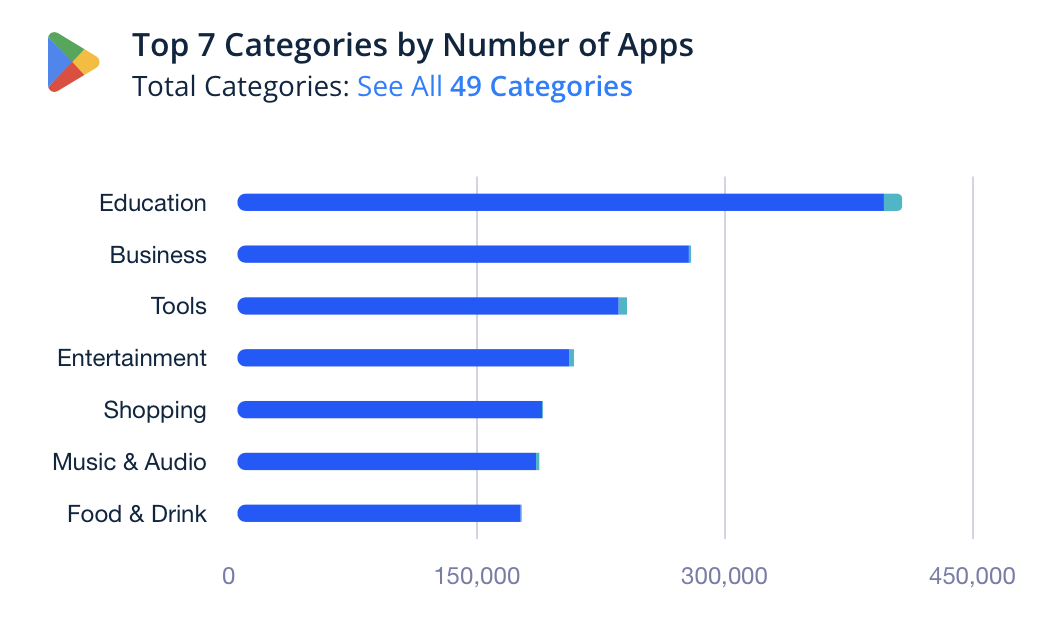
\includegraphics[width=\linewidth]{img/intro/google_play_categories.png}
\caption{Apps por categoría Google Play. Fuente: \href{https://42matters.com/stats\#apps-by-category}{42matters}}
\label{fig:google_play}
\end{minipage}
\hfill
\begin{minipage}[t]{0.48\textwidth}
\centering
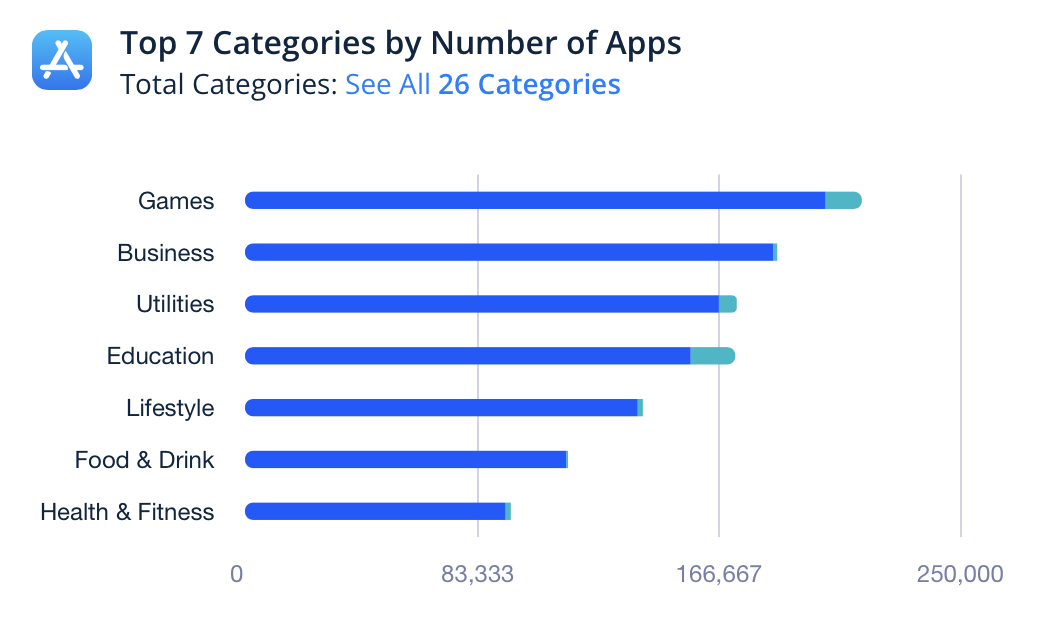
\includegraphics[width=\linewidth]{img/intro/app_store_categories.png}
\caption{Apps por categoría App Store. Fuente: \href{https://42matters.com/stats\#apps-by-category}{42matters}}
\label{fig:app_store}
\end{minipage}
\end{figure}

Además, se lanzan diariamente más de 2.300 nuevas aplicaciones en Google Play y unas 1.100 en App Store. Esto representa más de 90.000 aplicaciones nuevas al mes en la plataforma de Android, lo que pone de manifiesto la alta competencia y dinamismo de este mercado, Figura~\ref{fig:apps_per_month}.

\begin{figure}[H]
\centering
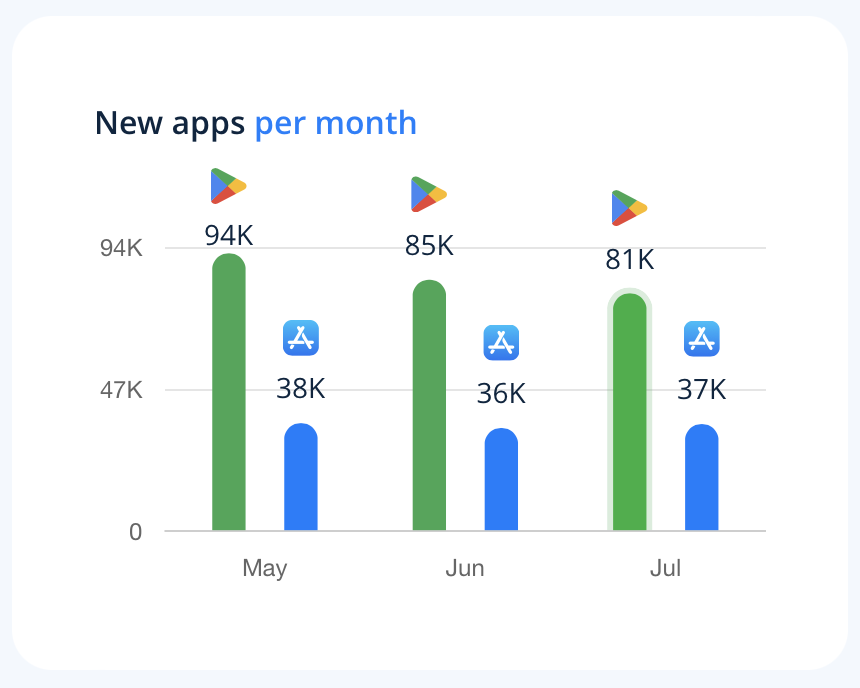
\includegraphics[width=0.6\textwidth]{./img/intro/apps_per_month.png}
\caption{Nuevas aplicaciones por mes en cada tienda de aplicaciones. Fuente: \href{https://42matters.com/stats\#apps-by-category}{42matters}}
\label{fig:apps_per_month}
\end{figure}

En cuanto a los sistemas operativos más utilizados, como se puede ver en la Figura~\ref{fig:world_map_ios_android}, Android domina el panorama global (no tiene en cuenta dispositivos tablets). Según Statista (junio de 2024), su cuota de mercado alcanza el 72,15\%, frente al 27,19\% de iOS. Aunque en países como Estados Unidos e Irlanda iOS tiene más presencia, Android es el sistema operativo predominante en regiones como América Latina, África, Asia y, especialmente, España.

\begin{figure}[H]
\centering
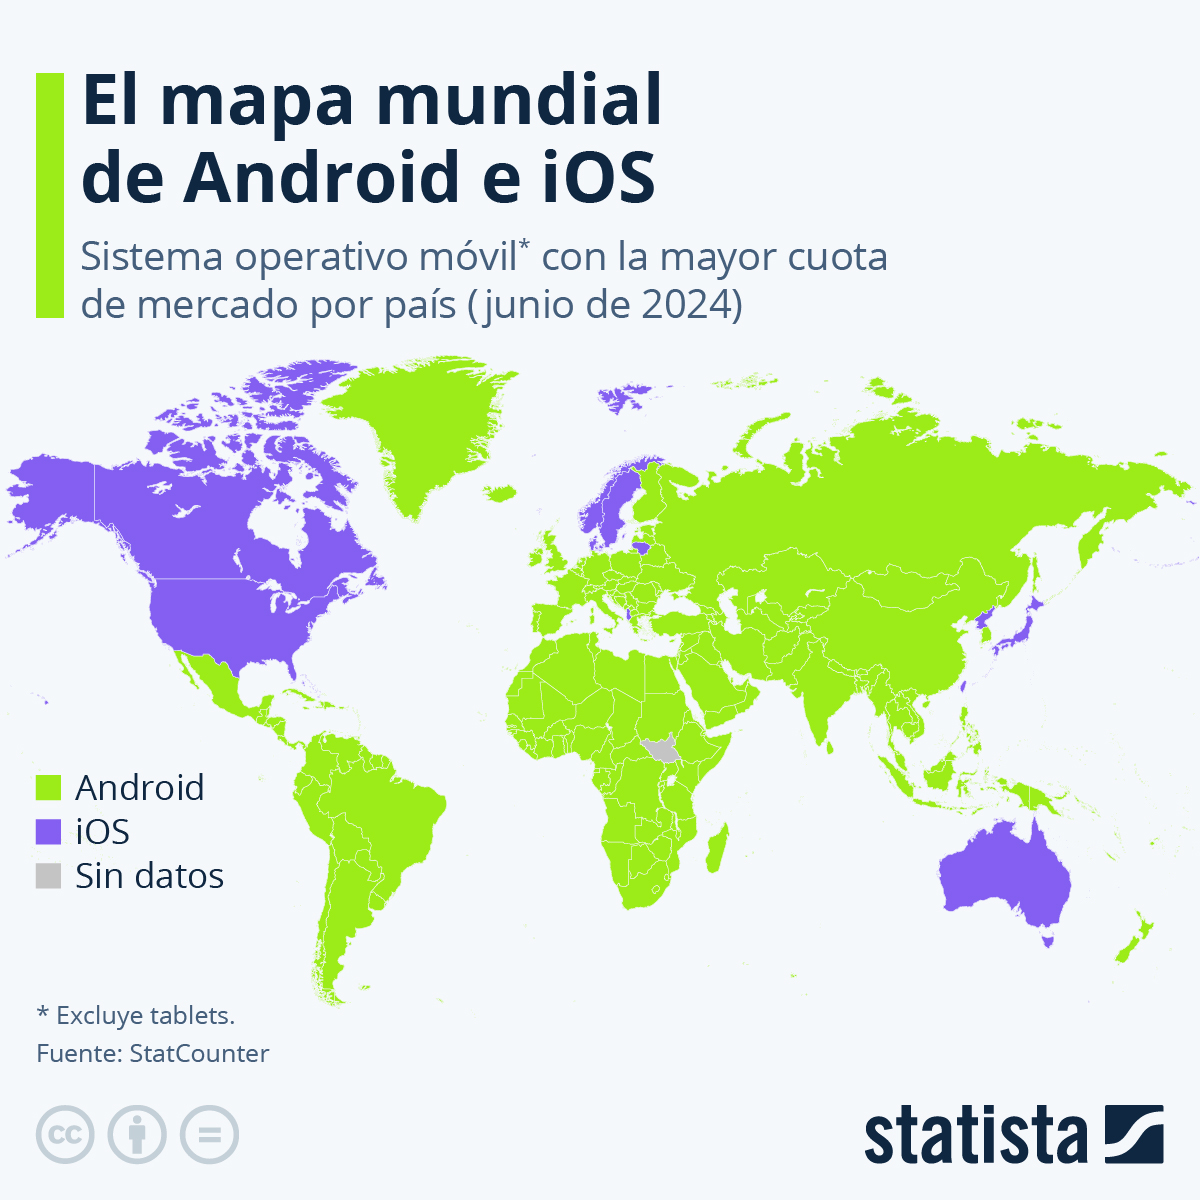
\includegraphics[width=0.6\textwidth]{./img/intro/world_map_ios_android.jpeg}
\caption{Mapa mundial de Android e iOS.  Fuente: \href{https://www.statista.com}{Statista}}
\label{fig:world_map_ios_android}
\end{figure}

En el caso concreto de España, que es donde se publicaría esta aplicación, el 77\% de los smartphones son Android frente a un 23\% de iOS (Statista, diciembre 2023). Este dato resulta decisivo a la hora de seleccionar la plataforma de desarrollo, ya que permite orientar el producto a la mayoría de los usuarios potenciales.

\section{Tipos de aplicaciones móviles}

Se distinguen tres tipos principales: aplicaciones nativas, aplicaciones web y aplicaciones híbridas.

Una aplicación nativa es aquella que se crea específicamente para un sistema operativo móvil, utilizando su lenguaje y herramientas oficiales. Esto permite aprovechar al máximo las capacidades del hardware del dispositivo, lo que se traduce en un mayor rendimiento y más fluidez en la experiencia de usuario. Por ejemplo, se considera nativa una aplicación desarrollada en Kotlin para Android o en Swift para iOS. Su distribucción se realiza a través de su instalación desde plataformas oficiales como Google Play o App Store y, en caso de querer abarcar varios sistemas operativos, implica desarrollar una versión distinta para cada uno.

Las aplicaciones web, por el contrario, son páginas web optimizadas para dispositivos móviles, a las que se accede desde el navegador sin necesidad de instalación. Se desarrollan con tecnologías como HTML, CSS y JavaScript, y su principal ventaja es la portabilidad entre sistemas. Sin embargo, su rendimiento es inferior al de una aplicación nativa y tienen acceso limitado a las funcionalidades del dispositivo.

Las aplicaciones híbridas combinan elementos de ambas. Básicamente, se trata de aplicaciones web que se ejecutan dentro de un contenedor nativo, lo que permite distribuirlas desde tiendas oficiales y acceder a algunas funcionalidades del hardware. No obstante, la integración entre la parte web y la parte nativa puede ser compleja, sobre todo en términos de rendimiento y mantenimiento.

Tras analizar las características de cada enfoque, para este trabajo de fin de grado se optó por desarrollar una aplicación nativa Android. Esta decisión responde tanto al interés por aprender en profundidad el desarrollo específico para esta plataforma, como al deseo de ofrecer una experiencia más fluida, potente y adaptada a los dispositivos que predominan en el mercado español.

\section{Análisis del entorno}

Antes de iniciar el desarrollo de la aplicación, se llevó a cabo un análisis del entorno para identificar qué soluciones digitales existen.

Una de las aplicaciones más instaladas para la gestión de listas de la compra es \textit{Bring!}. Su funcionamiento se basa en la creación de listas de la compra mediante una interfaz visual con iconos organizados por categorías (frutas, lácteos, etc) y permite que varios usuarios participen en una lista. Sin embargo, no permite especificar cantidades con precisión, ni se integra con recetas o planificación semanal, lo que limita su utilidad para quienes desean gestionar la compra de forma más detallada.

En número de instalaciones le sigue de cerca \textit{Listonic}, con un diseño más clásico: listas de verificación con productos agrupados por su sección en el supermercado. Es rápida y práctica. No obstante, su interfaz resulta más básica y tampoco tiene en cuenta la planificación de menús, recetas o la personalización de listas según hábitos domésticos o eventos.

A diferencia de otras soluciones del mercado, Pinche aborda el problema de la organización de la compra doméstica desde una perspectiva práctica, personalizada y centrada en la realidad cotidiana de quienes gestionan los menús y las compras del hogar.

La aplicación se estructura en tres secciones: listas de la compra, recetas e invitados. En la sección de listas, el usuario puede crear múltiples listas adaptadas a distintas ocasiones —por ejemplo, “Lista semanal” o “Cumpleaños de María”— y añadir productos con su cantidad, e incluso el supermercado donde se prefiere comprarlos. En la sección de recetas, se puede incluir su elaboración detallada e ingredientes para un número determinado de comensales, además de añadir fácilmente esos ingredientes a cualquier lista activa si desea realizar la receta. Por último, en la sección de invitados, se puede registrar información personalizada sobre las personas que vienen a comer a casa, como sus intolerancias, preferencias y qué platos se les han preparado recientemente.

En definitiva, ofrece una solución que permite la planificación, optimizar el tiempo y evitar errores comunes como compras duplicadas, olvidos o preparación de menús inadecuados para los invitados.

Desde el punto de vista académico, el proyecto ofrece un caso completo para aplicar competencias clave del grado: desarrollo de interfaces modernas con Jetpack Compose, gestión de datos con Firebase, diseño orientado al usuario y trabajo bajo metodologías ágiles.

%%%%%%%%%%%%%%%%%%%%%%%%%%%%%%%%%%%%%%%%%%%%%%%%%%%%%%%%%%%%%%%%%%%%%%%%%%%%%%%%
% OBJETIVOS %
%%%%%%%%%%%%%%%%%%%%%%%%%%%%%%%%%%%%%%%%%%%%%%%%%%%%%%%%%%%%%%%%%%%%%%%%%%%%%%%%

\cleardoublepage % empezamos en página impar
\chapter{Objetivos} % título del capítulo (se muestra)
\label{chap:objetivos} % identificador del capítulo (no se muestra, es para poder referenciarlo)

El objetivo principal de este proyecto es comprender y aplicar todo el proceso que conlleva la creación de una aplicación desde cero. En este caso, nos centraremos en cómo facilitar al usuario la tarea de realizar la compra doméstica, tanto de alimentos como de productos del hogar, de manera eficiente y organizada. También se tendrá en cuenta cómo gestiona las recetas y los invitados que van a comer a su hogar.

Para ello el trabajo se centra en el desarrollo de una aplicación móvil nativa para el sistema operativo Android, denominada \textit{Pinche}.

La forma de alcanzar este objetivo consistirá en recorrer cada una de las etapas del proceso de desarrollo, adoptando los distintos roles que forman parte de un equipo digital: experiencia de usuario (UX), producto y desarrollo. Aunque el núcleo del trabajo se centrará en la parte técnica de desarrollo, también se tendrán en cuenta aspectos clave de diseño y definición del producto.

Adoptar esta perspectiva permite también tomar decisiones informadas a la hora de implementarla sobre las necesidades reales de los usuarios, los problemas que enfrentan en su día a día y cómo una solución tecnológica puede aportar valor real. Al asumir diferentes roles permite entenderemos los retos de la comunicación entre perfiles técnicos y no técnicos y la importancia de no perder el foco en el usuario final.

La motivación del proyecto radica tiene en cuenta también aplicar y reforzar conocimientos adquiridos durante el grado, desde el diseño de interfaces hasta la integración de servicios en la nube. Pero sin permanecer como técnicos o programadores aislados que no tienen el contexto del proyecto.

Desde ese punto de vista, el puramente técnico, se ha optado por utilizar tecnologías modernas del ecosistema Android: el lenguaje de programación Kotlin, el framework Jetpack Compose para la construcción de interfaces declarativas y los servicios de Firebase: Firestore como base de datos y Firebase Authentication para la gestión de usuarios. Estas tecnologías permiten un desarrollo flexible, escalable y están alineadas con las demandas actuales del sector.

Desde la perspectiva de diseño UX se ha adoptado una combinación de la metodología Design Thinking para la definición inicial del problema y el uso de la herramienta Figma para llevar acabo un diseño final intuitivo y que sea fácilmente iterable.

Por último, desde el lado de producto y gestión del proyecto, se aplica la metodología Lean Startup para validar hipótesis y metodologías ágiles como Scrum para organizar el desarrollo en iteraciones en Trello.

En resumen, el proyecto se plantea como una oportunidad para consolidar conocimientos técnicos, mejorar habilidades de diseño y comunicación, y resolver una necesidad real con impacto práctico.


%%%%%%%%%%%%%%%%%%%%%%%%%%%%%%%%%%%%%%%%%%%%%%%%%%%%%%%%%%%%%%%%%%%%%%%%%%%%%%%%
% TECNOLOGÍAS, HERRAMIENTAS Y METODOLOGÍAS %
%%%%%%%%%%%%%%%%%%%%%%%%%%%%%%%%%%%%%%%%%%%%%%%%%%%%%%%%%%%%%%%%%%%%%%%%%%%%%%%%

\cleardoublepage
\chapter{Tecnologías, Herramientas y Metodologías}

% Descripción de los lenguajes de programación, entornos de desarrollo, herramientas auxiliares, librerías de terceros, sistemas operativos, navegadores web, etc. utilizados para la realización del proyecto, así como la metodología empleada. El grado de profundidad a la hora de explicar cada tecnología dependerá de lo relevante que ha sido para el proyecto y lo conocida que es. Por ejemplo, si se usa el lenguaje de programación Java, no es necesario entrar en tanto detalle como si se usa un lenguaje mucho menos usado como Scala, por ejemplo.

% Respecto a la metodología, dada la naturaleza de los proyectos, se suele describir una metodología iterativa e incremental en espiral, en la que se van sucediendo reuniones con el profesor que van definiendo el ámbito del proyecto.

% Este capítulo puede tener una extensión entre 10 y 15 páginas.

\section{Lenguaje de programación}

Para implementar una aplicación nativa en Android se puede usar como lenguaje de programacion Java o Kotlin.
El desarrollo de Pinche se ha realizado utilizando Kotlin.

Las principales razones por las que se ha decidido usar Kotlin para el desarrollo de esta aplicación frente a Java son:

\begin{itemize}
    \item \textbf{Sintaxis más concisa y expresiva}: Kotlin permite reducir la cantidad de código, optimizando la Implementación. Por ejemplo, la gestión de getters/setters, estructuras de datos y operaciones sobre colecciones se realiza de forma mucho más directa y legible.

    \item \textbf{Seguridad frente a errores de null}: Kotlin incluye un sistema de tipos que distingue claramente entre referencias anulables y no anulables, lo que reduce la probabilidad de errores en tiempo de ejecución relacionados con punteros nulos (el conocido \textit{NullPointerException} en Java).

    \item \textbf{Interoperabilidad con Java}: Kotlin es totalmente interoperable con Java, lo que permite utilizar bibliotecas existentes. Esto es especialmente útil en Android, ya que muchas APIs aún están escritas en Java.

    \item \textbf{Compatibilidad con herramientas modernas de Android}: Kotlin se integra de forma nativa con bibliotecas modernas como Jetpack Compose, Hilt, Coroutines o Navigation, lo que simplifica el uso de arquitecturas modernas (como MVVM) y prácticas de desarrollo actuales.

    \item \textbf{Soporte oficial, comunidad y futuro garantizado}: Google ha declarado que “Android is Kotlin-first”, lo que coloca a Kotlin como lenguaje oficial recomendado.
\end{itemize}

\section{Frameworks y librerías}

\subsection{Jetpack Compose}

Para la construcción de la interfaz de usuario se ha utilizado \textbf{Jetpack Compose}, el framework de Android más moderno para crear interfaces de forma declarativa. Esta elección responde a usar herramientas actuales, recomendadas por Google, que permiten mayor productividad y fluidez en el desarrollo.

Durante mucho tiempo, el desarrollo de interfaces en Android se ha basado en el uso de archivos \texttt{XML} que describen los elementos de la interfaz de forma estática, combinados con código Java o Kotlin para enlazar y actualizar esos elementos en tiempo de ejecución. Este enfoque impone una separación forzada entre lógica e interfaz, y obliga a utilizar métodos como \texttt{findViewById()} o \texttt{ViewBinding}, lo que complica la sincronización entre los datos y la vista.

\textbf{Jetpack Compose} rompe con este modelo tradicional al introducir una forma de construir la UI de manera totalmente \textbf{declarativa}, es decir, describiendo \textit{qué} debe mostrarse en lugar de \textit{cómo} hacerlo paso a paso. La interfaz se define directamente en Kotlin, mediante funciones composables, lo que permite una mejor integración con la lógica de negocio, la reutilización de componentes y mejorar la legibilidad del código.

Entre las principales ventajas de Jetpack Compose frente a XML destacan:

\begin{itemize}
    \item \textbf{Menor complejidad}: No es necesario gestionar manualmente el enlace entre XML y código. La UI responde automáticamente a los cambios de estado.

    \item \textbf{Código más conciso y reutilizable}: Al trabajar con funciones de Kotlin, se pueden componer interfaces complejas a partir de pequeños componentes reutilizables.

    \item \textbf{Mejor integración con la arquitectura moderna}: Compose se integra de forma nativa con patrones como MVVM que es el que seguimos en este proyecto, flujos reactivos como StateFlow e incluso herramientas de testing específicas para UI.

    \item \textbf{Vista previa en tiempo real}: Android Studio permite visualizar cambios en la UI mientras se escribe el código, lo que acelera el diseño y validación de pantallas. A diferencia de XML con el que tienes que construir tu aplicación cada vez que quieras ver el impacto de un cambio.

    \item \textbf{Mantenimiento más sencillo}: Al eliminar el archivo XML y mantener toda la lógica en un solo lenguaje, se reduce el esfuerzo de mantenimiento y depuración.
\end{itemize}

%%EJEMPLO DE UN COMPONENTE COMPOSABLE %%CAPUTAS DE HILT en el siguiente apartado

\subsection{Jetpack Navigation}

Para la gestión de la navegación entre pantallas se ha utilizado \textbf{Jetpack Navigation}, que permite definir flujos de navegación mediante un grafo centralizado, asegurando la coherencia del estado de la aplicación y facilitando el paso de argumentos entre distintas pantallas y componentes.

%%CAPTURAS DE LA NAVEGACION?? %%CAPUTAS DE HILT en el siguiente apartado

\subsection{Hilt}

Con el objetivo de aportar robustex y escalabilidad a la aplicación, hemos recurrido a \textbf{Hilt} como sistema de \textit{inyección de dependencias}. Esto nos ha permitido simplificar la gestión de instancias y facilitar su sustitución por instancias de prueba para llevar a cabo los test. También se ha tenido en cuenta su integración con el ciclo de vida recomendado de Android y su compatibilidad con Jetpack.

%%CAPUTAS DE HILT en el siguiente apartado

\section{Firebase}

\textbf{Firebase}, de Google, es una plataforma de desarrollo de aplicaciones que proporciona una serie de servicios backend listos para usar: bases de datos en tiempo real, autenticación de usuarios, almacenamiento en la nube, análisis, herramientas de pruebas y despliegue. Está pensada especialmente para aplicaciones móviles y web. Su uso agiliza significamente el desarrollo del backend en aplicaciones.

En este proyecto se utilizan principalmente dos componentes clave de Firebase:

\begin{itemize}
    \item \textbf{Firebase Authentication:} permite implementar de forma sencilla el mecanismo de registro y acceso mediante email y contraseña que hemos utilizado en Pinche.

    \item \textbf{Cloud Firestore:} una base de datos NoSQL que permite almacenar y sincronizar datos en tiempo real entre los dispositivos de los usuarios y la nube, con una estructura basada en colecciones y documentos \cite{firestore}.
\end{itemize}

Una de las principales ventajas de Firebase es su integración nativa con Android, lo que simplifica su uso desde Kotlin, además de su escalabilidad y su soporte para herramientas de desarrollo como Android Studio y \textit{Firebase Emulator Suite}, que permite hacer pruebas locales de testeo sin impactar en la base de datos real.

\section{Entorno de desarrollo}

El entorno de desarrollo utilizado ha sido \textbf{Android Studio}, IDE oficial de Android. Proporciona herramientas avanzadas como el emulador y da soporte completo para Compose, Kotlin y Firebase. Para las pruebas de la app se han utilizado tanto emuladores como dispositivos físicos.

\section{Control de versiones}

Para la gestión del código fuente se ha utilizado el conocido sistema de control de versiones \textbf{Git} y \textbf{GitHub} como repositorio remoto. El trabajo se ha organizado siguiendo prácticas comunes en entornos colaborativos. Esto ha permitido mantener versiones estables y realizar integraciones progresivas de nuevas funcionalidades. El flujo de trabajo ha sido el siguiente: se han creado ramas para la implementación de tareas concretas, por ejemplo: \texttt{feature/login}, una vez finalizada la tarea y testeada de manera atómica su funcionalidad se mergea en la rama \texttt{dev} donde se comprueba que la nueva funcionalidad no afecta a las implementadas anteriormente y tras las comprobaciones se realiza la actualizacion de la rama \texttt{main} que es la rama estable del proyecto.

\section{Metodologías de desarrollo}

\subsection{Design Thinking}

Durante la fase inicial se aplicó el enfoque de \textbf{Design Thinking}, con especial énfasis en la definición del problema y centrada en el usuario objetivo. Su objetivo es generar soluciones de acuerdo con problemas detectados en un determinado marco de trabajo.   \cite{designthinking} \cite{designthinking-url}.

\subsection{Lean Startup}

\textbf{Lean Startup} es una metodología que ayuda al desarrollo de productos o servicios de manera ágil, reduciendo los riesgos, promoviendo el aprendizaje y disminuyendo el tiempo de lanzamiento. Todo esto contribuye también a reducir los gastos y riesgos, al situar al cliente real en el centro de todas las decisiones de desarrollo \cite{leanstartup}.

Los principios fundamentales de Lean Startup son:

\begin{itemize}
  \item \textbf{Producto Mínimo Viable (MVP)}: Se definen unas hipótesis a confirmar y se genera una versión básica del producto que cubra la funcionalidad necesaria para comprobar dichas hipótesis y redirigir la definición del producto según lo que funciona y lo que no.

  \item \textbf{Construir-Medir-Aprender}: Se construye el MVP, se mide su desempeño y aceptación por parte del usuario, se recopilan datos y se decide en base a ellos. Este ciclo se repite durante toda la definición del producto.

  \item \textbf{Experimentación continua}: Se evalúa constantemente el producto o servicio, de manera que no hay un plan fijo de acción ni se comprometen recursos desde el principio.

  \item \textbf{Iteraciones rápidas}: La generación de MVPs debe ser ágil, demostrando flexibilidad a la hora de aplicar los cambios necesarios tras la última iteración.

  \item \textbf{Validación de hipótesis}: Se utilizan métricas y datos que ayudan a vislumbrar si una idea de negocio tiene mercado o no, evitando el gasto innecesario de recursos.
\end{itemize}

\subsection{Agile}

La metodología \textbf{Agile} se centra en la flexibilidad, la colaboración y la entrega incremental de valor al cliente durante el desarrollo de un proyecto. Con esta metodología se pretende generar una mayor adaptabilidad frente a los cambios que surgen durante el desarrollo, reduciendo los tiempos de entrega y mejorando la calidad del producto.

Agile se basa en el \textit{Manifiesto Ágil}, publicado en 2001, que consta de cuatro valores principales y doce principios.

\paragraph{Valores del Manifiesto Ágil:}
\begin{itemize}
    \item Individuos e interacciones frente a procesos y herramientas.
    \item Software funcional sobre documentación extensiva.
    \item Colaboración con el cliente frente a negociación de contratos.
    \item Responder ágilmente al cambio frente a seguir un plan rígido.
\end{itemize}

\paragraph{Principios:}
\begin{itemize}
    \item Satisfacer al cliente mediante la entrega rápida y continua de software funcional.
    \item Aceptar los cambios, los requisitos por cumplir pueden ser incluidos en cualquier etapa del desarrollo.
    \item Entregar frecuentemente un producto funcional, en ciclos cortos de tiempo.
    \item Colaboración constante con el cliente para asegurar que se cubren todas sus necesidades.
    \item Motivar a los equipos de trabajo para fomentar su implicación y confianza.
    \item Comunicación cara a cara como medio más eficiente y efectivo.
    \item Valorar el software funcional como principal medida de progreso.
    \item Sostenibilidad mediante una velocidad constante y sostenible para que el ritmo al que trabaja el equipo sea accesible.
    \item Atención a la excelencia técnica y al buen diseño.
    \item Simplicidad, eliminando lo innecesario o lo que no aporta valor real.
    \item Equipos autoorganizados con capacidad de decisión.
    \item Revisión y ajuste constantes para mejorar la efectividad.
\end{itemize}

Algunas metodologías que surgen del enfoque Agile son \textbf{Scrum}, \textbf{Kanban} y \textbf{Extreme Programming (XP)}.

\paragraph{Scrum.} Es una metodología de trabajo que permite el manejo de proyectos complejos permitiendo que los equipos trabajen de manera iterativa e incremental. El trabajo se organiza en \textbf{Sprints}, que son ciclos cortos de tiempo que tienen como objetivo un incremento funcional del producto que el equipo está desarrollando.\cite{scrum}

Entre sus principales elementos dentro de la metodología Scrum encontramos roles claves como Product Owner, Scrum Master y el equipo de desarrollo. El \textbf{Product Owner} define cuáles son las prioridades que maximizan el valor del producto. El \textbf{Scrum Master} facilita el proceso Scrum y se asegura de que se aplica correctamente. Y, por último, el \textbf{equipo de desarrollo} es el encargado de implementar el producto.

Dentro de esta metodología también encontramos elementos o herramientas clave que facilitan su aplicación: \textbf{Product Backlog}, una lista priorizada de todas las tareas del proyecto, \textbf{Sprint Backlog}, que abarca todas las tareas a realizar en un sprint, y el \textbf{incremento} que sería el producto funcional que entrega el equipo de desarrollo al final de cada sprint.

Para la gestión del tiempo dentro de un sprint, Scrum recomienda realizar cuatro encuentros: Sprint Planning, Daily Scrum, Sprint Review y Sprint Retrospective. En el \textbf{Sprint Planning} el objetivo será planificar qué tareas, que deben ser atómicas, se van a desarrollar este sprint. Diariamente el progreso se coordinará en la sesión de \textbf{Daily Scrum}, será el momento de poner sobre la mesa posibles bloqueos que el equipo ha encontrado o los avances que ha ido realizando. Una vez finalizado el sprint tendremos el \textbf{Sprint Review} donde se revisará qué cantidad de trabajo ha sido realizado. Por último el \textbf{Sprint Retrospective}, una sesión en la que el equipo pueda reflexionar sobre cómo mejorar para el próximo Sprint.

\begin{figure}[H]
\centering
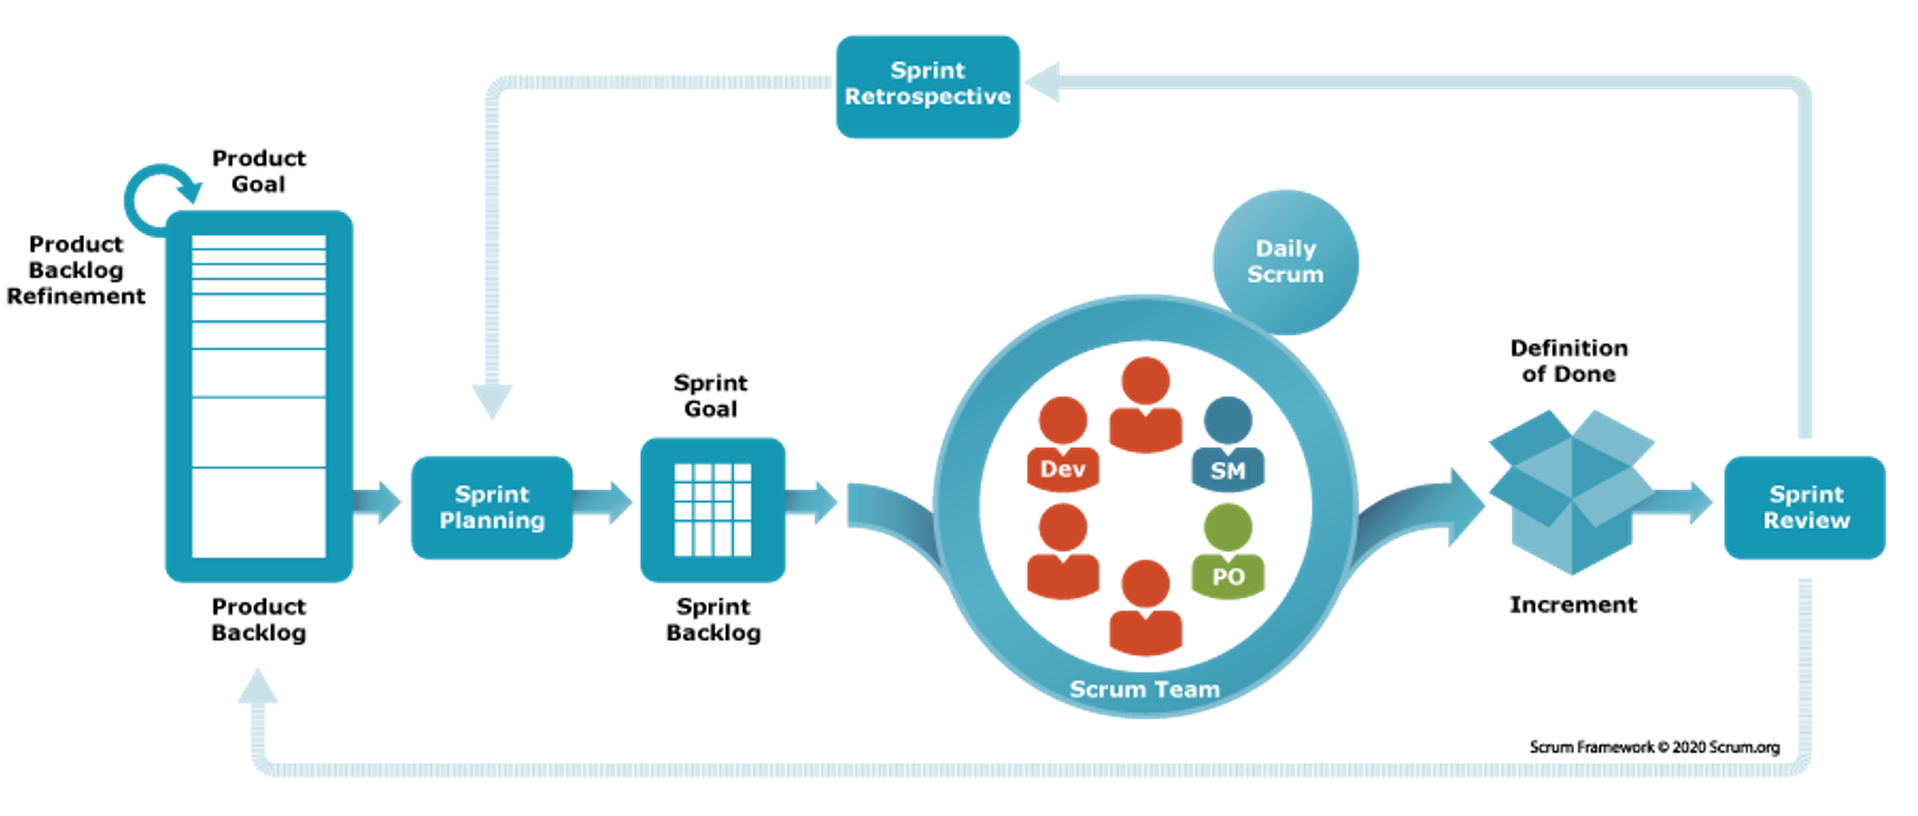
\includegraphics[width=0.9\textwidth]{./img/methodologies/scrum.png}
\caption{Esquema de funcionamiento de Scrum.}
\label{fig:scrum}
\vspace{0.2em}
{\footnotesize \centering \textit{Fuente:} \url{https://www.scrum.org/learning-series/what-is-scrum/} \par}
\end{figure}

\paragraph{Kanban.} Para esta metodología se suele utilizar un tablero visual (\textit{Tablero Kanban}) para representar el flujo de trabajo. Las tareas se representan como tarjetas que se mueven por columnas como \textit{Por hacer}, \textit{En progreso} y \textit{Terminado}. Se establece un límite de trabajo en curso (WIP: Work In Progress, trabajo en progreso) para evitar sobrecargas. Kanban permite detectar cuellos de botella, optimizar procesos y mejorar de forma continua la eficiencia del equipo.

\paragraph{Extreme Programming (XP).} XP enfatiza la mejora continua y la satisfacción del cliente. Reduce riesgos mediante prácticas técnicas rigurosas:

\begin{enumerate}
    \item Desarrollo iterativo con entregas frecuentes de software funcional.
    \item Pruebas constantes (TDD: Test-Driven Development, desarrollo guiado por tests).
    \item Programación en pareja. Dos desarrolladores trabajan simultáneamente en la misma tarea con el propósito de reducir errores y mejorar el aprendizaje del equipo.
    \item Integración continua.
    \item Código simple y funcional.
    \item Retroalimentación rápida del cliente. El cliente está presente de manera frecuente en el proceso de desarrollo y proporciona su punto de vista para ajustar el desarrollo a sus necesidades
\end{enumerate}

\section{Diseño de la interfaz}

La interfaz ha sido diseñada siguiendo principios de UX/UI centrados en la simplicidad, accesibilidad y claridad visual. Se han creado prototipos en Figma, permitiendo iterar sobre la estructura de navegación, la jerarquía visual y la organización de las secciones: listas, recetas e invitados.

\textbf{Figma} es una herramienta web de diseño de interfaces que permite crear prototipos interactivos, colaborar en tiempo real y compartir diseños entre equipos multidisciplinares. Es ampliamente utilizada en entornos de desarrollo ágil, ya que facilita la comunicación entre diseñadores, desarrolladores y clientes \cite{figma}.

\section{Herramientas de testeo}

Durante el desarrollo se han implementado diferentes tipos de tests para garantizar la calidad del producto, cada una con su propósito específico dentro del flujo de desarrollo. A continuación se describen los tipos principales de pruebas y las herramientas utilizadas en cada caso.

\subsection{Test unitarios}

Las pruebas unitarias se centran en comprobar el comportamiento de unidades individuales de código, normalmente funciones o clases, de forma aislada. Estas pruebas permiten validar la lógica de negocio sin dependencias externas.

\textbf{JUnit4} ha sido la herramienta principal para implementar los test unitarios en este proyecto \cite{android-testing}. Se trata del framework más consolidado en el ecosistema Java/Kotlin, ampliamente soportado y con buena integración en Android Studio. Junto a JUnit, se ha utilizado \textbf{MockK}, una librería de mocking especialmente diseñada para Kotlin, que permite simular dependencias como repositorios o servicios, da soporte para coroutines y se integra sin problema con los constructores Kotlin puros.

\subsection{Test de interfaz de usuario (UI)}

Los tests de UI tienen como objetivo comprobar que los componentes visuales se comportan correctamente frente a interacciones del usuario (clics, navegación, aparición de textos, etc.).

La libreria , específica para Jetpack Compose, ha sido la elegida para implementar este tipo de test en Pinche. Es una herramienta que permite simular eventos de usuario y verificar la presencia y el estado de los elementos de la pantalla \cite{android-testing}.

La ventaja frente a herramientas clásicas como Espresso para XML es que está optimizada para el modelo declarativo de Compose, lo que la hace más sencilla, menos propensa a errores de sincronización y mejor integrada con el ciclo de recomposición de la UI.

\subsection{Test de integración}

Los tests de integración validan el correcto funcionamiento de múltiples componentes combinados, como la lógica de presentación con la capa de datos.

Para este tipo de pruebas se ha utilizado \textbf{Firebase Emulator Suite}, una herramienta que permite simular servicios de Firebase (Firestore y Authentication en nuestro caso) localmente sin necesidad de acceder a entornos reales \cite{firebase-emulator}. Esto permite hacer pruebas reproducibles, seguras y con bajo coste.

Además, se han utilizado \textbf{repositorios falsos} (fakes) y la capacidad de Hilt para sustituir dependencias reales por versiones de prueba. Esto permite realizar pruebas sin tocar los datos reales ni alterar la lógica de producción.

Frente a enfoques como instrumentación real con dispositivos, esta estrategia ofrece mayor velocidad, control del entorno y testeo determinista.


% TENER EN CUENTA PARA FUTUROS CAMBIOS:

% \subsection{Test end-to-end (E2E)}

% Las pruebas de extremo a extremo comprueban flujos completos desde la interacción del usuario hasta la manipulación de datos, pasando por navegación, lógica de interfaz y persistencia.

% Para ello, se ha utilizado \textbf{Espresso}, el framework de referencia para pruebas E2E en Android \cite{android-testing}, junto con Firebase Emulator Suite para simular los servicios remotos.

% Espresso permite simular interacciones complejas del usuario, como navegación entre pantallas, introducción de texto y validación de mensajes en la interfaz. Aunque puede ser más lenta que otras pruebas, es fundamental para validar que todo el sistema funciona como un todo.

% \subsection{Test de cobertura}

% La cobertura de código permite conocer qué porcentaje del código ha sido ejecutado por las pruebas. Este indicador es útil para identificar posibles áreas no testeadas.

% En este proyecto se ha utilizado \textbf{JaCoCo}, una de las herramientas más utilizadas para generar informes de cobertura en proyectos Java y Kotlin \cite{jacoco}. JaCoCo se integra fácilmente con Gradle y genera reportes detallados con métricas por clase y método.

% Frente a otras opciones como Cobertura o Kotlin Coverage Plugin, JaCoCo ofrece una mejor integración con entornos Android y una comunidad de soporte más activa.

%%%%%%%%%%%%%%%%%%%%%%%%%%%%%%%%%%%%%%%%%%%%%%%%%%%%%%%%%%%%%%%%%%%%%%%%%%%%%%%%
% DESCRIPCIÓN INFORMÁTICA %
%%%%%%%%%%%%%%%%%%%%%%%%%%%%%%%%%%%%%%%%%%%%%%%%%%%%%%%%%%%%%%%%%%%%%%%%%%%%%%%%

\cleardoublepage
\chapter{Descripción informática}

Descripción del proyecto realizado. Después de unos párrafos introductorios el capítulo se divide en subcapítulos. (de 25 a 35 páginas)

\section{Requisitos}
\label{sec:requisitos}

Descripción detallada de las funcionalidades que tendría que implementar la aplicación (pues se asume que los requisitos se escriben antes de empezar el desarrollo). Pueden tener forma de historias de usuario o bien ser una lista de requisitos funcionales y no funcionales.

\section{Arquitectura y Análisis}
\label{sec:arquitectura-analisis}

Descripción de los aspectos de alto nivel de la aplicación. Diagramas de clases de análisis, diagramas de clases de diseño, etc. Se debe incluir la suficiente información para que el lector pueda entender la estructura de alto nivel del software desarrollado. Se pueden incluir diagramas de casos de uso si se considera útil.

\section{Diseño e Implementación}
\label{sec:diseno-implementacion}

Descripción de algún aspecto relevante de la implementación que quiera mencionarse. Por ejemplo se podría incluir alguno de los siguientes aspectos:
\begin{itemize}
  \item Algoritmo complejo que se haya tenido que desarrollar.
  \item Integración entre librerías problemática.
  \item Resolución de algún bug que haya sido especialmente problemático.
  \item Focalizar en alguna parte del desarrollo y describirla en más detalle.
\end{itemize}

En esta sección se pueden incluir fragmentos de código fuente. También se pueden incluir algunas métricas del proyecto (número de clases, líneas de código, etc.). También se puede incluir la evolución del repositorio de GitHub (gráfico de commits por día).

\section{Pruebas}
\label{sec:pruebas}

En esta sección se describen las pruebas automáticas que han sido implementadas para el proyecto. Sobre los tests, conviene indicar la cobertura del código. Si no se han implementado pruebas automáticas, deberían haberse implementado y describirse aquí o tener una buena justificación de por qué no se han implementado.


\section{Requisitos}
\label{sec:requisitos}

La aplicación \textbf{Pinche} nace con el objetivo de facilitar la organización de la compra doméstica mediante una herramienta móvil accesible, intuitiva y práctica. Para ello, se han definido una serie de requisitos funcionales que reflejan las necesidades del usuario final, así como requisitos no funcionales que garantizan la calidad del sistema.

\subsection{Requisitos funcionales}

Para definir los requisitos funcionales se ha seguido una metodolog\'ia personalizada que combina las fortalezas de las metodolog\'ias \textbf{Scrum}, \textbf{Kanban} y \textbf{Extreme Programming (XP)}. Se ha seguido la estructura iterativa de Scrum, utilizando tableros Kanban para visualizar el flujo de tareas y adoptando buenas pr\'acticas como pruebas continuas e integraci\'on frecuente propias de XP.

La organizaci\'on del desarrollo ha comenzado con la definici\'on de \textbf{historias de usuario}, expresadas en el formato: ``Como [tipo de usuario], quiero [funcionalidad] para [beneficio]''. Estas historias fueron elaboradas y refinadas por el equipo de desarrollo en conjunto con el Product Owner, y se han estimado mediante la t\'ecnica de \textbf{Story Points} basada en la sucesi\'on de Fibonacci (1, 2, 3, 5, 8, 13).

Las historias se han agrupado en \textbf{\'epicas}, agrupaciones l\'ogicas que organizan funcionalidades principales: \textit{Cuenta de usuario}, \textit{Lista de la compra}, \textit{Recetas} e \textit{Invitados}.


La épica \textit{Cuenta de usuario} agrupa un total de seis historias de usuario con sus respectivas tareas que tienen como objetivo toda la gestión dentro de la aplicación de la cuenta del usuario. Las historias de usuario serian:

\begin{enumerate}
  \item Como usuario, necesito registrarme en la aplicación con la finalidad de poder utilizarla. Estimación: 2 puntos de historia.
  \item Como usuario, necesito iniciar sesión en la aplicación con la finalidad de acceder a mi cuenta de usuario y mis datos. Estimación: 1 punto de historia.
  \item Como usuario, necesito cerrar sesión en la aplicación con la finalidad de no dejar mi cuenta activa en un dispositivo. Estimación: 1 punto de historia.
  \item Como usuario, quiero recuperar mi contraseña de mi cuenta de usuario de la aplicación con la finalidad de poder acceder a mi cuenta. Estimación: 1 punto de historia.
  \item Como usuario, quiero ver un resumen de mi actividad con la finalidad de conocer cuál es mi uso de la aplicación. Estimación: 2 puntos de historia.
  \item Como usuario, necesito eliminar mi cuenta de usuario de la aplicación con la finalidad de borrar mis datos y dejar de tener cuenta de usuario en la aplicación. Estimación: 1 punto de historia.
\end{enumerate}

La épica \textit{Lista de la compra} agrupa un total de trece historias de usuario con sus respectivas tareas que tienen como objetivo toda la gestión dentro de la aplicación de las listas de la compra y la gestión de sus respectivos artículos. Las historias de usuario serian:

\begin{enumerate}
  \item Como usuario, quiero ver el listado de las listas de la compra que he creado con la finalidad de saber cuántas y qué listas de la compra tengo. Estimación: 2 puntos de historia.
  \item Como usuario, quiero ver el listado de listas de la compra que aún no han sido completadas con la finalidad de poder visualizar más fácilmente que listas tienen artículos por comprar. Estimación: 1 punto de historia.
  \item Como usuario, quiero acceder al detalle de una lista de la compra en concreto con la finalidad de ver sus artículos. Estimación: 1 punto de historia.
  \item Como usuario, quiero eliminar una lista de la compra, aunque haya sido o no completada, con la finalidad de dejar de visualizarla en mi listado. Estimación: 1 punto de historia.
  \item Como usuario, quiero seleccionar como comprados todos los artículos de una lista de la compra con la finalidad de poder completar una lista en un solo click. Estimación: 1 punto de historia.
  \item Como usuario, quiero seleccionar como pendientes de comprar todos los artículos de una lista con la finalidad de volver a reutilizar esa lista. Estimación: 1 punto de historia.
  \item Como usuario, quiero añadir una nueva lista de la compra con la finalidad de tener una nueva lista donde organizar mis artículos. Estimación: 1 punto de historia.
  \item Como usuario, quiero añadir un artículo a una lista de la compra con la finalidad de recordar que tengo que comprar dicho artículo. Estimación: 1 punto de historia.
  \item Como usuario, quiero seleccionar un artículo como comprado con la finalidad de poder visualizar qué artículos ya he comprado. Estimación: 1 punto de historia.
  \item 	Como usuario, quiero seleccionar un artículo que ya había seleccionado como comprado como no comprado en una lista de la compra con la finalidad de poder volver a tener ese artículo como pendiente de comprar. Estimación: 1 punto de historia.
  \item Como usuario, quiero eliminar un artículo de una lista de la compra con la finalidad de dicho artículo deje de formar parte de la lista de la compra. Estimación: 1 punto de historia.
  \item Como usuario, quiero especificar el nombre del artículo, la cantidad, la unidad de medida de esa cantidad, la tienda donde prefiero comprar y opcionalmente una fotografía del artículo, con la finalidad de disponer de toda la información que necesito de ese artículo. Estimación: 2 puntos de historia.
  \item Como usuario, quiero editar la información de un artículo de una lista de la compra con la finalidad de modificar su contenido. Estimación: 1 punto de historia.
\end{enumerate}

La épica \textit{Recetas} agrupa un total de ocho historias de usuario con sus respectivas tareas que tienen como objetivo toda la gestión dentro de la aplicación de las recetas que genere el usuario. Las historias de usuario serian:

\begin{enumerate}
  \item Como usuario, quiero ver un listado con mis recetas con la finalidad de conocer que recetas tengo registradas. Estimación: 2 puntos de historia.
  \item Como usuario, quiero añadir una nueva receta desde la pantalla de listas de recetas con la finalidad de añadir una nueva receta y sus datos. Estimación: 1 punto de historia.
  \item Como usuario, quiero editar una receta con la finalidad de actualizar datos de esa receta. Estimación: 1 punto de historia.
  \item Como usuario, quiero eliminar una receta con la finalidad de que no aparezca esa receta en mi listado de recetas. Estimación: 1 punto de historia.
  \item Como usuario, quiero acceder a la información de una receta desde la pantalla de lista de recetas con la finalidad de ver en detalle los datos de esa receta. Estimación: 1 punto de historia.
  \item Como usuario, quiero añadir información a una nueva receta con la finalidad de tener toda su información recopilada. Estimación: 2 puntos de historia.
  \item Como usuario, quiero editar la información de una receta con la finalidad de tener la información de esa receta actualizada. Estimación: 1 punto de historia.
  \item Como usuario, quiero eliminar una receta con la finalidad de eliminar esa receta de mis recetas. Estimación: 1 punto de historia.
\end{enumerate}

La épica \textit{Invitados}, agrupa un total de ocho historias de usuario con sus respectivas tareas que tienen como objetivo toda la gestión dentro de la aplicación de los invitados que añada el usuario a su lista de invitados. Las historias de usuario serian:

\begin{enumerate}
  \item Como usuario, quiero ver un listado con mis invitados con la finalidad de conocer que invitados tengo registrados. Estimación: 2 puntos de historia.
  \item Como usuario, quiero añadir un nuevo invitado desde la pantalla de listas de invitados con la finalidad de añadir un nuevo invitado y sus datos. Estimación: 1 punto de historia.
  \item Como usuario, quiero editar un invitado con la finalidad de actualizar datos de ese invitado. Estimación: 1 punto de historia.
  \item Como usuario, quiero eliminar un invitado con la finalidad de que no aparezca ese invitado en mi listado de invitados. Estimación: 1 punto de historia.
  \item Como usuario, quiero acceder a la información de un invitado desde la pantalla de lista de invitados con la finalidad de ver en detalle los datos de ese invitado. Estimación: 1 punto de historia.
  \item Como usuario, quiero añadir información a un nuevo invitado con la finalidad de tener toda su información recopilada. Estimación: 2 puntos de historia.
  \item Como usuario, quiero editar la información de un invitado con la finalidad de tener la información de ese invitado actualizada. Estimación: 1 punto de historia.
  \item Como usuario, quiero eliminar un invitado con la finalidad de eliminar ese invitado de mis invitados. Estimación: 1 punto de historia.
\end{enumerate}

Una vez refinadas y estimadas, se ha preparado el primer Sprint de dos semanas de duraci\'on. Se ha fijado un l\'imite de 13 puntos de historia por Sprint. En este primer ciclo, se priorizaron historias de cada \'epica para implementar las funcionalidades b\'asicas. Sin embargo, solo se completaron 6 de las 8 historias planificadas debido a la carga de requisitos no funcionales que se requeria implementar en este primer Sprint.

El seguimiento del Sprint se ha realizado mediante un tablero \textbf{Kanban} creado en \textbf{Trello}, donde se representan las historias como tarjetas con sus tareas asociadas. La Figura~\ref{fig:user_story_trello} muestra cómo se define una historia de usuario en Trello y la Figura~\ref{fig:final_sprint_trello} el estado final del tablero en el primer Sprint.

\begin{figure}[H]
\centering
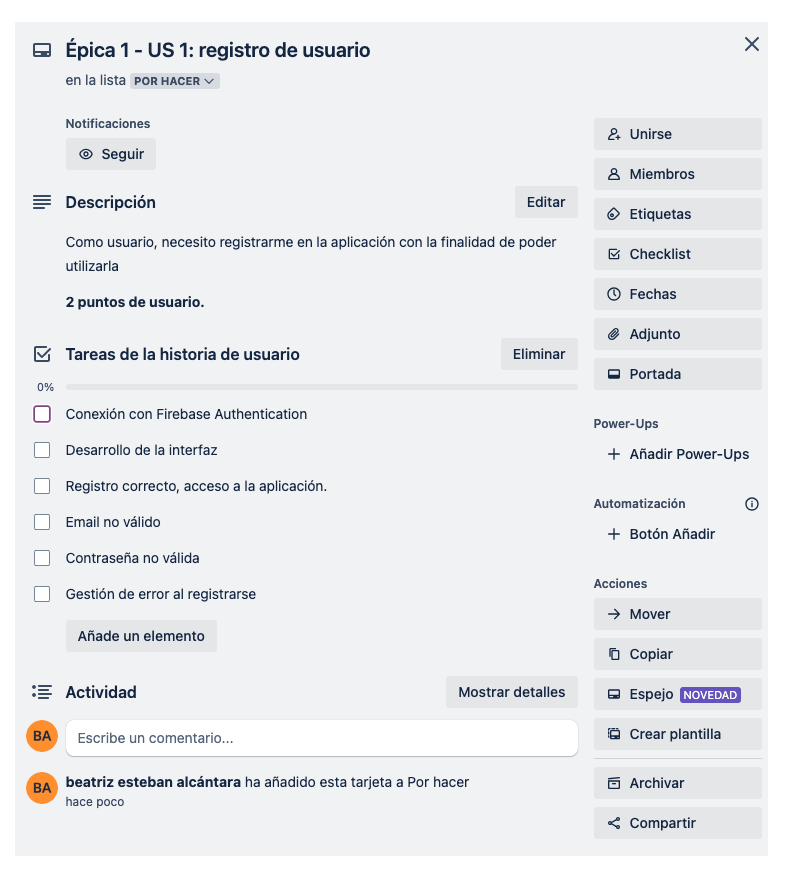
\includegraphics[width=0.6\textwidth]{./img/requirements/user_story_trello.png}
\caption{Historia de usuario en Trello}
\label{fig:user_story_trello}
\end{figure}

\begin{figure}[H]
\centering
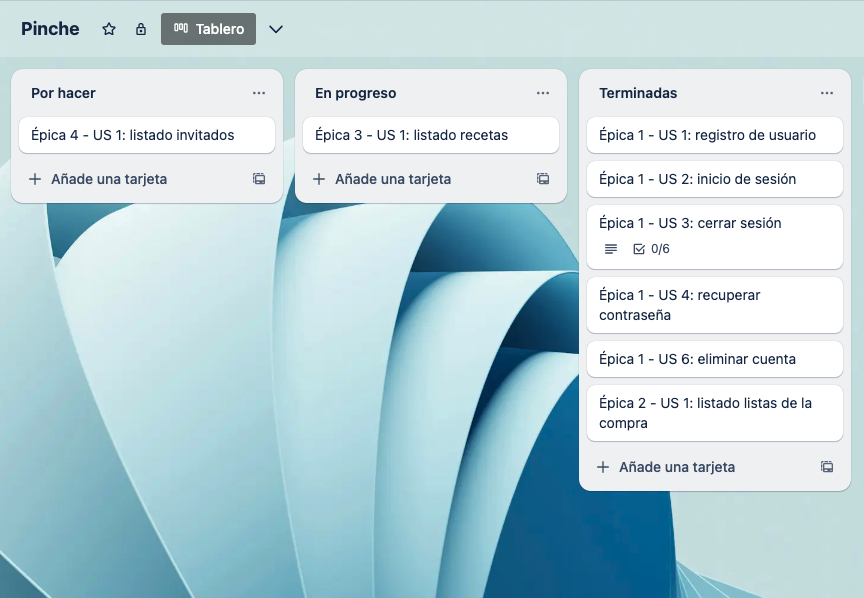
\includegraphics[width=0.6\textwidth]{./img/requirements/final_sprint_trello.png}
\caption{Estado del tablero Kanban al final del primer Sprint.}
\label{fig:final_sprint_trello}
\end{figure}

Tras la sesión de \textit{Sprint Review} y la de \textit{Sprint Retrospective}, se ajust\'o el alcance estimado para los siguientes Sprints a un m\'aximo de 8 puntos de historia por iteraci\'on, adaptando as\'i la velocidad al contexto real del desarrollo.

Una hoja resumen con todas las historias de usuario, agrupadas por \'epica, sus tareas y estimaciones, se adjunta en el anexo \texttt{Historias de usuario.xlsx}.

\subsection{Requisitos no funcionales}

Además de la funcionalidad, se han establecido los siguientes requisitos no funcionales:

\begin{itemize}
    \item \textbf{Aplicación nativa Android}, desarrollada con \textbf{Kotlin} y \textbf{Jetpack Compose}, para garantizar buen rendimiento y aprovechamiento de los recursos del dispositivo \cite{kotlin,jetpack}.
    \item \textbf{Persistencia de datos en la nube} mediante \textbf{Firebase Firestore} para facilitar el acceso a la información desde diferentes dispositivos \cite{firestore}.
    \item \textbf{Autenticación de usuarios} mediante \textbf{Firebase Authentication}, garantizando un sistema de acceso seguro y sencillo \cite{firebase-auth}.
    \item \textbf{Interfaz centrada en la experiencia de usuario}, basada en los principios de diseño de Google Material Design.
    \item \textbf{Estructura modular y escalable}, basada en el patrón arquitectónico \textbf{MVVM} (Model-View-ViewModel).
\end{itemize}

Estos requisitos definen el alcance funcional y técnico del proyecto, garantizando que el producto final responda tanto a las expectativas del usuario como a criterios de calidad del software.


\section{Arquitectura y análisis}
\label{sec:arquitectura-analisis}

La arquitectura de una aplicación móvil resulta crítica para garantizar su escalabilidad, optimización del código, rendimiento, solidez, mantenibilidad,y la correcta separación de responsabilidades. En este proyecto se ha adoptado la arquitectura recomendada por Android, basada en una estructura en capas y el patrón MVVM (Model-View-ViewModel), con la inclusión de una capa de dominio opcional y la gestión de dependencias mediante Hilt.

\subsection{Principios generales}

Esta arquitectura promueve los principios de separación de responsabilidades, flujo unidireccional de datos, modularidad y testabilidad \cite{android-architecture}. El modelo propuesto divide la lógica de la aplicación en tres capas principales: UI, dominio (opcional) y datos, Figura~\ref{fig:mvvm}. En nuestro caso vamos a utilizar la arquitectura recomendada incluyendo la capa opcional de dominio.

\begin{figure}[H]
\centering
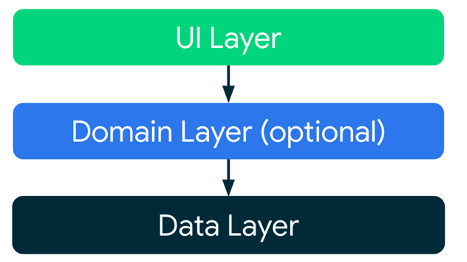
\includegraphics[width=0.6\textwidth]{./img/mvvm.png}
\caption{Diagrama arquitectura MVVM.}
\label{fig:mvvm}
\vspace{0.2em}
{\footnotesize \centering \textit{Fuente:} \url{https://developer.android.com/topic/architecture?hl=es-419} \par}
\end{figure}

\subsection{Capa de UI}

La capa de interfaz de usuario es responsable de mostrar los datos al usuario y recoger sus interacciones. Esta capa se compone de dos tipos de elementos:

\begin{itemize}
    \item \textbf{Elementos de la UI}: Son funciones de Jetpack Compose que renderizan los datos en pantalla.
    \item \textbf{Contenedores de estado}: Los ViewModel que retienen el estado de la UI y exponen datos reactivos mediante \texttt{StateFlow}.
\end{itemize}

\subsection{Capa de dominio}

La capa de dominio encapsula la lógica empresarial que puede ser compartida entre distintos ViewModels. En ella se definen los casos de uso (\textit{use cases}) como clases que representan acciones o procesos específicos de la aplicación, facilitando la reutilización de código y la claridad del flujo de datos.

\subsection{Capa de datos}

Esta capa es responsable de la obtención y persistencia de datos, ya sea desde fuentes remotas como Firebase Firestore, o locales. Se organiza en:

\begin{itemize}
    \item \textbf{Repositorios}: Actúan como intermediarios entre las fuentes de datos y la capa de dominio.
    \item \textbf{Fuentes de datos}: Pueden ser locales o remotas. En nuestro caso, son remotas: usamos Firebase que proporciona servicios de autenticación y base de datos en la nube \cite{firestore, firebase-auth}.
\end{itemize}

Gracias a esta separación, si en el futuro se quisiera cambiar de base de datos (por ejemplo, de Firebase a Amazon DynamoDB), solo se vería afectada la capa de datos, manteniendo intacto el resto del sistema.

\subsection{Gestión de dependencias con Hilt}

La gestión de dependencias se realiza mediante la biblioteca Hilt, un contenedor de inyección de dependencias desarrollado por Google. Hilt proporciona objetos preconfigurados a las clases de Android y administra automáticamente su ciclo de vida \cite{hilt-android}. Esto permite:

\begin{itemize}
    \item Reducir el acoplamiento entre componentes.
    \item Facilitar el testeo gracias a la posibilidad de sustituir dependencias reales por versiones simuladas.
    \item Garantizar la escalabilidad del código mediante una configuración declarativa y reutilizable.
\end{itemize}

\subsection{Ventajas de esta arquitectura}

La aplicación Pinche se beneficia de esta arquitectura al conseguir:

\begin{itemize}
    \item Mejor separación de responsabilidades entre componentes.
    \item Mayor facilidad de testeo en todas las capas.
    \item Reutilización de lógica empresarial entre distintas pantallas.
    \item Facilidad para mantener y escalar el código base en el futuro.
\end{itemize}

Este enfoque permite un desarrollo estructurado, coherente y sostenible, favoreciendo además la implementación de buenas prácticas de ingeniería de software.


\section{Diseño e implementación}
\label{sec:diseno-implementacion}

El desarrollo de la aplicación \textbf{Pinche} se ha centrado en aplicar buenas prácticas de ingeniería de software para Android, incluyendo el patrón MVVM, el uso de Jetpack Compose y la organización modular del código.

\subsection{Análisis de requerimientos y estructura funcional}

La aplicación ha sido diseñada en base a un conjunto de funcionalidades organizadas en tres secciones principales: listas de la compra, recetas e invitados. Este enfoque permite abordar de forma modular las necesidades de los usuarios y facilita la extensión del sistema.

El modelo de datos se ha estructurado para cubrir las siguientes entidades principales:

\begin{itemize}
    \item \textbf{Lista}: contiene un conjunto de productos, su nombre y estado.
    \item \textbf{Producto}: asociado a una lista, con nombre, cantidad y supermercado.
    \item \textbf{Receta}: incluye nombre, pasos de elaboraci\'on, ingredientes y número de comensales.
    \item \textbf{Ingrediente}: definido por nombre y cantidad relativa a los comensales.
    \item \textbf{Invitado}: con nombre, preferencias alimentarias, intolerancias y registro de comidas anteriores.
\end{itemize}

Este modelo facilita la integración de funcionalidades como el cálculo de ingredientes según el número de comensales, la generación de listas automáticas a partir de recetas y la personalización de menús para invitados con restricciones.

\subsection{Patr\'on MVVM}

El patrón Model-View-ViewModel (MVVM) permite una clara separación de responsabilidades entre la interfaz de usuario y la lógica de negocio. Esta estructura permite un mejor testeo, una mayor mantenibilidad del código y una arquitectura reactiva orientada al ciclo de vida del sistema \cite{viewmodel}.

\begin{itemize}
    \item \textbf{Model}: representa la capa de datos de la aplicación, incluyendo los repositorios y el acceso a Firestore.
    \item \textbf{View}: implementada usando Jetpack Compose, se encarga de mostrar los datos y de capturar la interacción del usuario.
    \item \textbf{ViewModel}: contiene la lógica de presentación, retiene el estado y orquesta el flujo de datos entre View y Model usando \texttt{StateFlow}.
\end{itemize}

\subsection{Jetpack Compose y su integraci\'on}

Jetpack Compose es el framework de UI moderno de Android, que permite declarar interfaces de forma reactiva con funciones de Kotlin \cite{jetpack}. Gracias a su enfoque declarativo, se reduce la cantidad de código boilerplate y se mejora la legibilidad del código fuente.

Ejemplo de composable en la aplicación:

\begin{verbatim}
@Composable
fun RecipeCard(recipe: Recipe) {
    Card(modifier = Modifier.padding(8.dp)) {
        Column {
            Text(text = recipe.name, style = MaterialTheme.typography.h6)
            Text(text = "Comensales: ${recipe.servings}")
        }
    }
}
\end{verbatim}

\subsection{Decisiones técnicas relevantes}

Durante el desarrollo se tomaron decisiones clave como:

\begin{itemize}
    \item Uso de \textbf{Jetpack Navigation} para gestionar la navegación entre pantallas de manera estructurada.
    \item Implementación de \textbf{Hilt} para inyección de dependencias, facilitando el testeo y la escalabilidad.
    \item Empleo de \textbf{StateFlow} para la gestión del estado de la UI, evitando fugas de memoria.
    \item Utilización de \textbf{Git} como sistema de control de versiones, junto con ramas por tarea y buenas prácticas de integración continua (CI).
    \item Desarrollo colaborativo organizado a través de tableros \textbf{Trello} y prototipos creados en \textbf{Figma}.
\end{itemize}

Esta implementación modular y centrada en buenas prácticas garantiza que Pinche pueda mantenerse y escalarse en el tiempo, facilitando la extensi\'on de funcionalidades futuras.

\section{Pruebas}
\label{sec:pruebas}

El aseguramiento de la calidad en el desarrollo de la aplicación \textbf{Pinche} se ha abordado mediante una estrategia de pruebas estructurada que cubre distintos niveles de validación del sistema: pruebas unitarias, de interfaz, de integración, de extremo a extremo (E2E) y cobertura de código. Esta estrategia ha permitido verificar que los componentes funcionan correctamente de forma individual y en conjunto.

\subsection{Pruebas unitarias}

Las pruebas unitarias validan pequeñas unidades de código de forma aislada, principalmente funciones puras o clases sin dependencias externas. Para ello se ha utilizado \textbf{JUnit4} como framework base, complementado con \textbf{MockK} para simular comportamientos de dependencias externas como repositorios o servicios \cite{android-testing}.

MockK se ha elegido frente a otras alternativas como Mockito debido a su compatibilidad nativa con Kotlin, su soporte para coroutines y su sintaxis más idiomática.

el Listado~\ref{lst:signinTest},

\begin{lstlisting}[language=Java, caption={SignInUserUseCaseTest}, label={lst:signinTest}]
  @ExperimentalCoroutinesApi
  class SignInUserUseCaseTest {

    @get:Rule
    val coroutinesTestRule = MainDispatcherRule()

    private val authRepository: AuthRepository = mockk()
    private lateinit var signInUserUseCase: SignInUserUseCase

    private val email = "test@example.com"
    private val password = "123456"

    @Before
    fun setup() {
        signInUserUseCase = SignInUserUseCase(authRepository)
    }

    @Test
    fun `sign in returns Success when repository succeeds`() = runTest {
        coEvery { authRepository.firebaseSignInWithEmailAndPassword(email, password) } returns Success(true)

        val result = signInUserUseCase(email, password)

        assertTrue(result is Success)
        coVerify { authRepository.firebaseSignInWithEmailAndPassword(email, password) }
    }

    @Test
    fun `sign in returns Failure when repository fails`() = runTest {
        val exception = Exception("Auth error")
        coEvery { authRepository.firebaseSignInWithEmailAndPassword(email, password) } returns Failure(exception)

        val result = signInUserUseCase(email, password)

        assertTrue(result is Failure)
        coVerify { authRepository.firebaseSignInWithEmailAndPassword(email, password) }
    }
}
\end{lstlisting}

\subsection{Pruebas de interfaz (UI)}

Para comprobar el comportamiento de la interfaz de usuario, se ha utilizado la librería \texttt{androidx.compose.ui:ui-test-junit4}, integrada en Jetpack Compose. Esta herramienta permite verificar la presencia de elementos, sus estados, y simular acciones del usuario como clics o introducción de texto.

Frente a otras librerías tradicionales como Espresso, esta herramienta ofrece mejor sincronización con el ciclo de recomposición de Compose y facilita pruebas más declarativas \cite{android-testing}.

\subsection{Pruebas de integración}

Las pruebas de integración validan que múltiples componentes trabajen juntos de forma coherente. En este proyecto se han utilizado:

\begin{itemize}
    \item \textbf{Firebase Emulator Suite}, que simula los servicios de Firebase (Firestore y Auth) localmente \cite{firebase-emulator}.
    \item \textbf{Repositorios simulados} combinados con \textbf{Hilt} para sustituir dependencias reales durante las pruebas.
\end{itemize}

Este enfoque permite realizar pruebas realistas pero controladas, sin depender de servicios externos ni afectar datos en producción.

\subsection{Pruebas end-to-end (E2E)}

Las pruebas E2E verifican que la aplicación funciona correctamente en su conjunto, desde la interacción del usuario hasta el acceso a datos y navegación.

Se ha empleado \textbf{Espresso}, el framework oficial de Google para pruebas E2E en Android, junto con Firebase Emulator Suite para simular los servicios remotos. Estas pruebas son útiles para validar flujos completos como el inicio de sesión, la creación de listas o la adición de productos \cite{android-testing}.

\subsection{Cobertura de código}

Como métrica adicional de calidad, se ha utilizado \textbf{JaCoCo} para generar informes de cobertura de código. Esto permite conocer qué líneas del proyecto han sido ejecutadas durante las pruebas y detectar zonas sin cobertura suficiente \cite{jacoco}.

JaCoCo se integra fácilmente con Gradle y Android Studio, proporcionando estadísticas precisas que se han utilizado para ajustar el alcance de las pruebas implementadas.


%%%%%%%%%%%%%%%%%%%%%%%%%%%%%%%%%%%%%%%%%%%%%%%%%%%%%%%%%%%%%%%%%%%%%%%%%%%%%%%%
% CONCLUSIONES Y TRABAJOS FUTUROS %
%%%%%%%%%%%%%%%%%%%%%%%%%%%%%%%%%%%%%%%%%%%%%%%%%%%%%%%%%%%%%%%%%%%%%%%%%%%%%%%%

\cleardoublepage
\chapter{Conclusiones y trabajos futuros}
\label{chap:conclusiones-trabajos-futuros}

% Reflexión sobre el trabajo realizado, qué objetivos se han cumplido y qué aspectos quedan pendientes para una futura ampliación del proyecto. Además, se deben incluir unas conclusiones personales indicando lo que ha supuesto para el alumno la realización del trabajo. Entre 2 y 4 páginas.

\section{Objetivos cumplidos}
\label{sec:objetivos-cumplidos}
En esta sección voy a diferenciar dos objetivos claros que se han presentado a lo largo de este proyecto.

En primer lugar, comprender y analizar las funciones y responsabilidades de cada rol en un equipo digital. Se ha cumplido el objetivo de explorar y aplicar metodologías y herramientas conmunmente utilizadas por el equipo de diseño y de producto, de las que desde el lado técnico solemos tener menos compresión pero que impactan directamente en nuestro trabajo. Y por supuesto, refrescar y aplicar todo el conocimiento adquirido durante la realización del grado que aplica a estos dos roles. Esto ha permitido dar una solución centrada en el usuario para facilitar una tarea tan cotidiana y personalizable como la gestión de la compra en el hogar.

Y en segundo lugar, la exploración de todas las tecnologías y buenas prácticas que actualmente aplican al desarrollo de aplicaciones nativas, especialmente de Android. Al entenderlas, otro de los objetivos cumplidos ha sido saber conocer qué opciones hay y cómo aplicar las que realmente eran necesarias o aportaban un valor en el desarrollo de Pinche.

Tanto en el prototipo funcional en figma como en la planificación de historias de usuario que se plantea en la etapa inicial de este proyecto, hay una discrepancia entre lo planteado y lo que se ha llegado a implementar en la aplicación.

Cumpliendo con toda la funcionalidad prevista para las secciones de gestión de la cuenta del usuario en la aplicación y de la lista de la compra con sus respectivos articulos. Pero sin llegar a implementar por completo las funcionalidades de gestión de recetas (incluir detalles a la receta y añadir sus artículos en una lista de la compra) y de invitados (incluir detalles del invitado y añadir las recetas que se le han preparado y sus favoritas). Esto se debe a una estimación que no preveía el tiempo y esfuerzo requerido para adquirir y aplicar conocimientos nuevos en un campo tan amplio como el desarrollo nativo de aplicaciones.

\section{Trabajos futuros}
\label{sec:trabajos-futuros}

Tras la implementación de una base sólida de la aplicación Pinche, las líneas de trabajo futuro que considero que tendría sentido implementar son:

\begin{itemize}
    \item \textbf{Funcionalidades planteadas pero no implementadas:} Terminar de implementar la gestión completa de recetas e invitados.
    \item \textbf{Internalización:} Añadir la opción de cambiar de idioma dentro de la aplicación, ampliando así el mercado de posibles usuarios.
    \item \textbf{Incorporación de fotografías:} Ofrecer la opción de añadir fotografías de los artículos, de las recetas y de los invitados.
    \item \textbf{Incorporar funcionalidades gracias a la Inteligencia Artificial (IA):} Explorar cómo la IA puede impactar en nuevas funcionalidades en la aplicación. Por ejemplo, recomendar alimentos o recetas al usuario o predecir el gasto de un alimento para añadirlo de nuevo a la lista de la compra.
    \item \textbf{Accesibilidad:} Incluir todo el código necesario para que la aplicación sea accesible para todos los usuarios: etiquetas de accesibilidad, cambio de diseño, etc.
    \item \textbf{Ampliar la cobertura de tests:} Terminar por cubrir por completo la aplicación con los tests unitarios ya planteados y añadir tests de interfaz y tests de extremo a extremo (E2E). Los tests E2E comprueban flujos completos: desde la interacción del usuario, la navegación, el estado de la interfaz, la manipulación de los datos y la persistencia de los mismos. Incorporar también tests de cobertura que permitan conocer qué porcentaje de código se testea en las pruebas.
\end{itemize}

\section{Conclusiones personales}
\label{sec:conclusiones-personales}

La realización de este trabajo me ha permitido conocer la complejidad y los beneficios de realizar un proyecto siguiendo buenas prácticas desde la definición a la implementación pasando por la etapa de diseño y el control del progreso.

He entendido las dificultades que sufren equipos multidisciplinares digitales para comunicarse y la importancia de entender las decisiones de cada rol. Creo que es una parte fundamental y que facilita el trabajo de un desarrollador a parte de conocer, entender e implementar correctamente las tecnologias actuales y las buenas prácticas de generación de código. En mi opinión, la comunicación entre roles es una habilidad que en cualquier empresa del sector o en cualquier proyecto que se realiza en equipo hay que aplicar, cuidar y mejorar.

Ha sido mi primer contacto con la implementación de una aplicación nativa en Android. Puede que aprender el lenguaje de programación Kotlin y el comprender y aplicar buenas prácticas como: la arquitectura MVVM, la inyección de dependencias, la navegación, el estado de los componentes de Jetpack Compose o realización de test unitarios haya sido la parte a la que más tiempo he dedicado y que más esfuerzo me ha requerido. Sin embargo, como siempre pasa con las buenas prácticas, me he beneficiado de aplicar todas ellas durante todo el desarrollo de la aplicación.

He aprendido muchos conceptos que impactan por completo en mi carrera profesional, añadiendo a mis conocimientos de desarrollo Front-End la parte nativa de aplicaciones, que tiene una alta demanda en el sector, abriéndome así las puertas a nuevas oportunidades de empleo y de desarrollo en mi carrera profesional.

%%%%%%%%%%%%%%%%%%%%%%%%%%%%%%%%%%%%%%%%%%%%%%%%%%%%%%%%%%%%%%%%%%%%%%%%%%%%%%%%
% BIBLIOGRAFÍA %
%%%%%%%%%%%%%%%%%%%%%%%%%%%%%%%%%%%%%%%%%%%%%%%%%%%%%%%%%%%%%%%%%%%%%%%%%%%%%%%%

\cleardoublepage

\bibliographystyle{abbrv}
\bibliography{memoria}

%%%%%%%%%%%%%%%%%%%%%%%%%%%%%%%%%%%%%%%%%%%%%%%%%%%%%%%%%%%%%%%%%%%%%%%%%%%%%%%%
% APÉNDICE(S) %
%%%%%%%%%%%%%%%%%%%%%%%%%%%%%%%%%%%%%%%%%%%%%%%%%%%%%%%%%%%%%%%%%%%%%%%%%%%%%%%%

\cleardoublepage
\appendix
\chapter{Manual de usuario}
\label{app:manual}

\end{document}
